%
% File emnlp2015.tex
%
% Contact: daniele.pighin@gmail.com
%%
%% Based on the style files for ACL-2015, which were, in turn,
%% Based on the style files for ACL-2014, which were, in turn,
%% Based on the style files for ACL-2013, which were, in turn,
%% Based on the style files for ACL-2012, which were, in turn,
%% based on the style files for ACL-2011, which were, in turn,
%% based on the style files for ACL-2010, which were, in turn,
%% based on the style files for ACL-IJCNLP-2009, which were, in turn,
%% based on the style files for EACL-2009 and IJCNLP-2008...

%% Based on the style files for EACL 2006 by
%%e.agirre@ehu.es or Sergi.Balari@uab.es
%% and that of ACL 08 by Joakim Nivre and Noah Smith

\documentclass[11pt,a4paper]{article}
\usepackage{acl2015}
\usepackage{times}
\usepackage{url}
\usepackage{latexsym}
\usepackage{graphicx}
\usepackage{amsmath}

%\setlength\titlebox{5cm}

% You can expand the titlebox if you need extra space
% to show all the authors. Please do not make the titlebox
% smaller than 5cm (the original size); we will check this
% in the camera-ready version and ask you to change it back.


\title{Sentiment Analysis of Amazon Product Reviews Using Domain Adversarial Training}

\author{First Author \\
  Affiliation / Address line 1 \\
  Affiliation / Address line 2 \\
  Affiliation / Address line 3 \\
  {\tt email@domain} \\\And
  Second Author \\
  Affiliation / Address line 1 \\
  Affiliation / Address line 2 \\
  Affiliation / Address line 3 \\
  {\tt email@domain} \\}

\date{}

\begin{document}
\maketitle
\begin{abstract}
  In this project, sentiment analysis of Amazon product reviews was
  done across three different domains(viz. books, music and dvd). We
  have used domain adversarial training for the neural network.
\end{abstract}

\section{Introduction}

We have tried to develop a sentiment classifier in this project for product reviews scraped from Amazon while addressing the problem of Domain Adaptation. This means that our classifier learns in the presence of a shift in the domains of training and testing environments. We achieve this by training a domain and sentiment classifier together using Adverserial training. In this approach, the loss of sentiment classifier is minimized while that of the domain classifier is maximized so that the sentiment predictions are made independent of domain. We first experiment with a straightforward CNN classifier to define a baseline performance and then modify the network by adding domain adverserial training to it.

We will also explore the following research questions:
\begin{itemize}
  \item Training procedure.
  \item Effect of Optimizers (Dhruv)
  \item Effect of Activation functions (Ishan)
\end{itemize}

\section{Classification with CNN}

We take the model described in ~\cite{Britz} as the baseline and modify it to train on our dataset. It looks like Figure ~\ref{fig:figure1}. The first layer converts words into embedding vectors. The next layer performs convolutions over the embedded word vectors using multiple filter sizes. Next, we max-pool the result of the convolutional layer into a long feature vector, add dropout regularization, and classify the result using a softmax layer.

\begin{figure}[htb]
\begin{center}
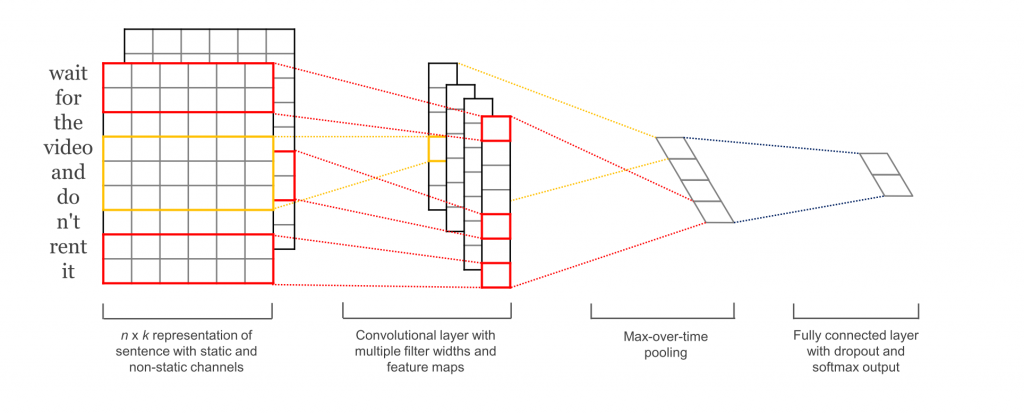
\includegraphics[width=\columnwidth]{cnn.png}
\end{center}
\caption{Image source: ~\cite{Britz}}
\label{fig:figure1}
\end{figure}

We trained different models on all domains (books, dvd, music) and then evaluated them on all the domains. Table ~\ref{cnn-table} gives a summary of the accuracies calculated on test set. Rows mean that a given dataset is evaluated on different models. Columns mean that a given model is evaluated on different data sets. Therefore, for row "books" and column "dvd" means that the model trained on "dvd" is evaluated on "books". As expected, the model performs best when both the training and testing domain is the same. The accuracies are thus the highest across the diagonal. This model uses "ReLU" as the activation and "Adam" as the optimizer.


\begin{table}[h]
\begin{center}
\begin{tabular}{|l|l|l|l|}
\hline \bf & \bf Books & \bf Dvd & \bf Music \\ \hline
Books & 0.766 & 0.7325 & 0.6815 \\
Dvd & 0.7165 & 0.756 & 0.7105 \\
Music & 0.709 & 0.7455 & 0.77 \\
\hline
\end{tabular}
\end{center}
\caption{ Training results for baseline CNN }
\label{cnn-table}
\end{table}



\section{Domain Adversarial Training}

We followed the approach based on domain adaptation described in ~\cite{Ganin:2016} paper.
In this approach, neural network architectures that are trained on labeled data from
the source domain and unlabeled data from the target domain. As the training continues,
the procedure encourages prominence of features that are biased towards for the main
learning task on the source domain and unbiased towards the shift between the domains.

\subsection{Domain Adversarial Neural Network Architecture}
\begin{figure}[htb]
\begin{center}
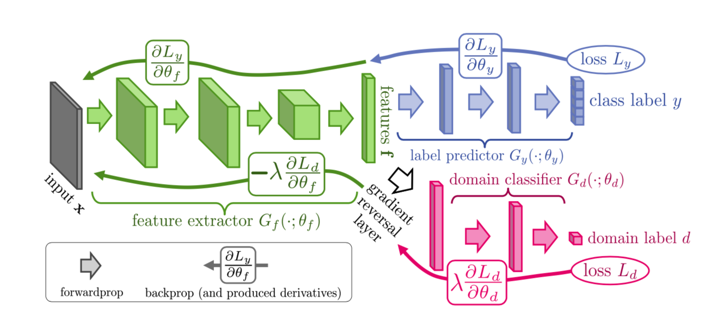
\includegraphics[width=\columnwidth]{dann.png}
\end{center}
\caption{Domain Adversarial Training Neural Network, Image source: ~\cite{Ganin:2016}}
\label{fig:figure2}
\end{figure}

The architecture includes feature extractor(green), label predictor(blue) and domain classifier(red). In Layer 1,  we convert the input sentences into vector space using using word embedding from GLoVe. This outputs a matrix for each review. In Layer 2 and 3,  we use CNN and then max-pool to convert input matrix into a column vector.  In Layer 4, single layer with activation function (feature extractor). In Layer 5 and 6, single layer with softmax with feature extractor output as the input to both layers.

\subsection{Our Approach}
\begin{figure}[htb]
\begin{center}
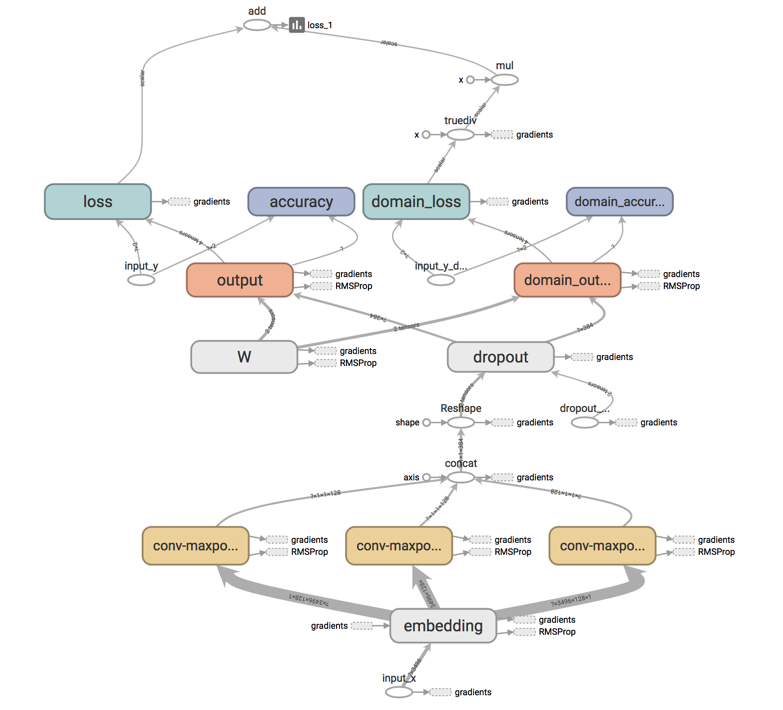
\includegraphics[width=\columnwidth]{tensorflow_nn.png}
\end{center}
\caption{Our Neural Network viewed on Tensorboard}
\label{fig:figure3}
\end{figure}

Our objective is to minimize the label loss and maximise the domain loss. We tried a couple of ways to achieve this and we report two techniques which worked the best.

\subsubsection{Approach 1}
We have introduced a hyperparameter in the network named domain\_loss\_factor\_propagation i.e. we include a percentage of domain loss in the in the total loss at every step time. In this way, our network tries to minimize the combined loss of label prediction loss along with small factor of domain classification loss. The loss equation being minimised is:
\begin{itemize}
  \item label\_loss + domain\_loss\_factor\_propagation*(1/domain\_loss)
\end{itemize}


\subsubsection{Approach 2}
We introduce a different hyperparameter named domain\_train\_frequency. In this scheme, we train the randomly train either the label network or the domain network based on the hyperparameter value. The following values are minimised:

\begin{itemize}
  \item (1/domain\_loss) randomly "domain\_train\_frequency" times out of the total training steps
  \item label\_loss otherwise
\end{itemize}

\subsection{Research Question: Effect of Activation Functions}
Activation functions which are easily differentiable and easy to train should be used in neural networks. To briefly describe the purpose of activation functions is to add the non-linearity to the neural networks. So we trained the network for the two approaches described above using four different types of activation functions: [ReLU, Tanh, ELU and Softplus].
We used stardard implementations provided in Tensorflow with all the default parameters. The experiments section describes the a comparative analysis of the performance of different activation functions named above.

Brief description of the described activation functions are as follows:-
\subsubsection{ReLU}
$f(x)= \max(0,x), f'(x) = \begin{cases}
      0 & x < 0 \\
      1 & x\geq 0 \\
   \end{cases}$

The ReLU is the most used activation function in the world right now. Since, it is used in almost all the convolutional neural networks or deep learning. But the issue is that all the negative values become zero immediately which decreases the ability of the model to fit or train from the data properly. That means any negative input given to the ReLU activation function turns the value into zero immediately in the graph, which in turns affects the resulting graph by not mapping the negative values appropriately.
\begin{figure}[htb]
\begin{center}
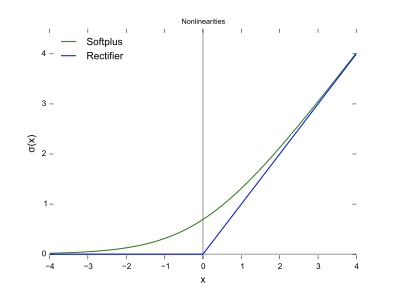
\includegraphics[width=\columnwidth]{Rectifier_and_softplus_functions.png}
\end{center}
\caption{ReLU and Softplus curve }
\label{fig:figure4}
\end{figure}

\subsubsection{Softplus}
$f(x)= \log(1+\exp{x}), f'(x) = \frac{1}{1+exp{-x}}$

Softplus is a newer function than Sigmoid and Tanh. It is firstly introduced in 2001. Softplus is an alternative of traditional functions because it is differentiable and its derivative is easy to demonstrate.

\subsubsection{Tanh}
\begin{figure}[htb]
\begin{center}
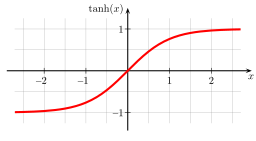
\includegraphics[width=\columnwidth]{Hyperbolic_Tangent.png}
\end{center}
\caption{Tanh curve}
\label{fig:figure5}
\end{figure}
$f(x) = \tanh(x), f'(x) = 1-f(x)^2$

Tanh function is s-shaped.The advantage is that the negative inputs will be mapped strongly negative and the zero inputs will be mapped near zero in the Tanh graph.

\subsubsection{ELU}

$f(x)= \begin{cases}
      \alpha*((\exp{x})-1) & x < 0 \\
      x & x\geq 0 \\
   \end{cases},$

$f'(x) = \begin{cases}
      f(x)+\alpha & x < 0 \\
      1 & x\geq 0 \\
   \end{cases}$
\begin{figure}[htb]
\begin{center}
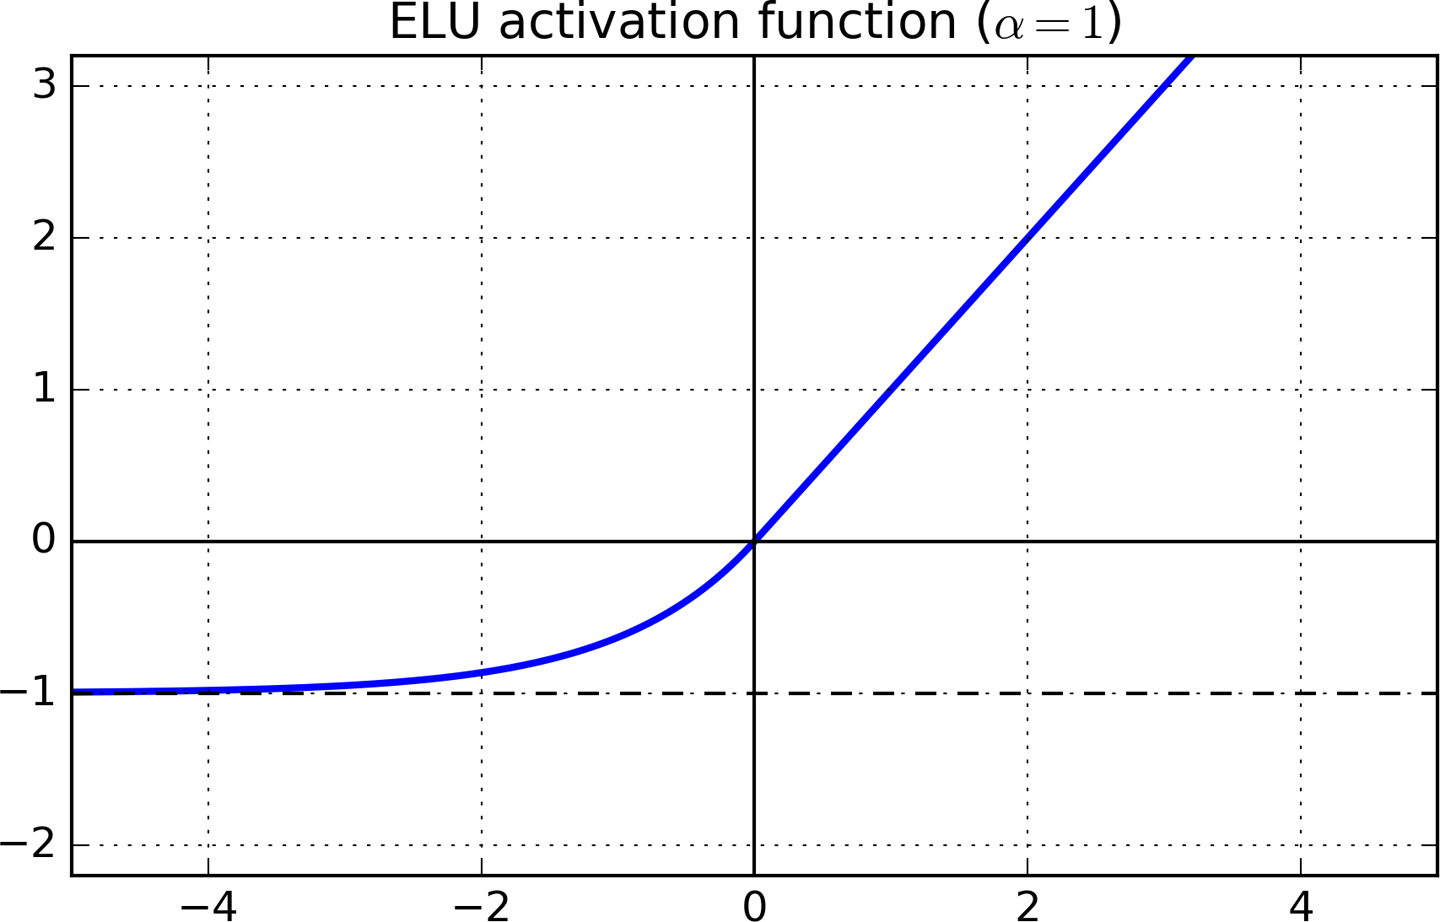
\includegraphics[width=\columnwidth]{elu.png}
\end{center}
\caption{ELU curve}
\label{fig:figure6}
\end{figure}

ELU is very similiar to ReLU except negative inputs. They are both in identity function form for non-negative inputs. On the other hand, ELU becomes smooth slowly until its output equal to -α whereas ReLU sharply smoothes. Different to other activation functions, ELU has a extra alpha constant which should be positive number.

\subsection{Research Question: Optimizers}
We trained the network for the two approaches described above using two different types of gradient descent optimizers: RMSprop and Adam. To briefly describe them, RMSprop divides the gradient by a running average of its recent magnitude while Adam in addition also uses the average of the second moments of the gradients.

We used stardard implementations provided in Tensorflow with all the default parameters except epsilon (which is a small constant provided for avoiding zero denominator) which given a value of 1e-3. The loss equation used is as stated in the two approaches above.

A detailed description of how the optimization algorithm works is beyond the scope of this work. The experiments section describes the a comparative analysis of the performance of using optimizers.


\section{Dataset}
The data is from 3 different domains (books, dvds, movies) and 3 different languages (German, English, French).
We have only used the English dataset for this work. The data has been obtained from: \url{https://www.uni-weimar.de/en/media/chairs/computer-science-and-media/webis/corpora/corpus-webis-cls-10/} and it is described in~\cite{PB:2010}.

For each language and each domain there are 2000 training examples and 2000 test examples. The ratings to positive/negative sentiment are mapped as follows: 1.0, 2.0: negative, 4.0, 5.0: positive. There are no instances with a rating of 3.0. The datasets are balanced, this means for each language and each domain 50\% of the items have a positive and 50\% have a negative rating.

\section{Experiments and Results}
Table~\ref{alpha-activation-table} and~\ref{1d-activation-table} compare the accuracies for networks trained using Adam as the optimizer and changing the activation functions from the set[ReLU, Tanh, ELU and Softplus] for different values of hyperparameters named domain\_loss\_factor\_propagation and domain\_train\_frequency. As can be seen, Softplus clearly outperforms every other activation functions.

Another pattern which emerges from the tables is that son increasing the values, the performance gets deteriorated. For example, in Table ~\ref{1d-activation-table}, the value of 0.2 for domain\_train\_frequency results in no learning at all because the network is making random guesses. Due to this reason, we did not train every other activation functions except ReLU for this value.

Table ~\ref{alpha-optimizer-table} and ~\ref{1d-optimizer-table} compare the accuracies for networks trained using ReLU as the activation function and changing the optimizers between Adam and RMSprop for different values of hyperparameters named domain\_loss\_factor\_propagation and domain\_train\_frequency. As can be seen, RMSprop clearly outperforms Adam.

Another pattern which emerges from the tables is that slightly higher values of hyperparameters completely destroy the performance. For example, in Table ~\ref{1d-optimizer-table}, the value of 0.2 for domain\_train\_frequency results in no learning at all because the network is making random guesses. Due to this reason, we did not train RMSprop for this value.

\begin{table}[h]
\begin{center}
\begin{tabular}{|c|l|l|l|l|}
\hline
Activation & \multicolumn{1}{|p{1cm}|}{Domain loss \%}& Books & Dvd & Music \\
\hline
ReLU & 0.05 & 0.7375 & 0.756 & 0.715  \\
 & 0.1 & 0.741 & 0.7465 & 0.703 \\
 & 0.2 & 0.742 & 0.7435 & 0.7155 \\
\hline
tanh & 0.05 & 0.755 & 0.7655 & 0.7255 \\
 & 0.1 & 0.75 & 0.7515 & 0.7035 \\
 & 0.2 & 0.741 & 0.7355 & 0.7145 \\
\hline
ELU & 0.05 & 0.7395 & 0.7515 & 0.712 \\
 & 0.1 & 0.75 & 0.7515 & 0.727 \\
 & 0.2 & 0.7375 & 0.739 & 0.705 \\
\hline
Softplus & 0.05 & 0.7545 & 0.766 & 0.7335 \\
 & 0.1 & 0.7585 & 0.763 & 0.747 \\
 & 0.2 & 0.744 & 0.746 & 0.728 \\
\hline
\end{tabular}
\end{center}
\caption{ Training on books-music pair with domain loss factor propagation and activation functions with Adam Optimizer}
\label{alpha-activation-table}
\end{table}


\begin{table}[h]
\begin{center}
\begin{tabular}{|c|l|l|l|l|}
\hline
Activation & \multicolumn{1}{|p{1cm}|}{Domain train frequency}& Books & Dvd & Music \\
\hline
ReLU & 0.05 & 0.766 & 0.7775 & 0.737 \\
  & 0.1 & 0.7555 & 0.7585 & 0.7185 \\
  & 0.2 & 0.5 & 0.5 & 0.5 \\
\hline
tanh & 0.05 & 0.5 & 0.5 & 0.5  \\
  & 0.1 & 0.754 & 0.767 & 0.719 \\
\hline
ELU & 0.05 & 0.755 & 0.7675 & 0.737 \\
  & 0.1 & 0.746 & 0.766 & 0.731 \\
\hline
Softplus & 0.05 & 0.766 & 0.7675 & 0.7315 \\
  & 0.1 & 0.76 & 0.768 & 0.721 \\
\hline
\end{tabular}
\end{center}
\caption{ Training on books-music pair with domain train frequency and activation functions with Adam Optimizer}
\label{1d-activation-table}
\end{table}

\begin{table}[h]
\begin{center}
\begin{tabular}{|c|l|l|l|l|}
\hline
Activation & \multicolumn{1}{|p{1cm}|}{Domain loss \%}& Books & Dvd & Music \\
\hline
Adam & 0.05 & 0.7375 & 0.756 & 0.715 \\
 & 0.1 & 0.741 & 0.7465 & 0.703 \\
 & 0.2 & 0.742 & 0.7435 & 0.7155 \\
\hline
RMSprop & 0.05 & 0.781 & 0.7875 & 0.764 \\
 & 0.1 & 0.788 & 0.801 & 0.777 \\
\hline
\end{tabular}
\end{center}
\caption{ Training on books-music pair with domain loss factor propagation and optimizers with ReLU activation}
\label{alpha-optimizer-table}
\end{table}

\begin{table}[h]
\begin{center}
\begin{tabular}{|c|l|l|l|l|}
\hline
Activation & \multicolumn{1}{|p{1cm}|}{Domain train frequency}& Books & Dvd & Music \\
\hline
Adam & 0.05 & 0.766 & 0.7775 & 0.737 \\
 & 0.1 & 0.7555 & 0.7585 & 0.7185 \\
 & 0.2 & 0.5 & 0.5 & 0.5 \\
\hline
RMSprop & 0.05 & 0.784 & 0.7995 & 0.766 \\
 & 0.1 & 0.787 & 0.7995 & 0.7825 \\
\hline
\end{tabular}
\end{center}
\caption{ Training on books-music pair with domain train frequency and optimizers with ReLU activation}
\label{1d-optimizer-table}
\end{table}





\section{Conclusion}
We implemented the DANN based ~\cite{Ganin:2016} sentiment analysis and achieved better results with respect to the baseline model described in ~\cite{Britz} for the sentiment prediction. Hence the main task of DANN is achieved that is to learn a features which is predictive of the source example labels, but uninformative about the domain of the input (source or target)

Understanding activation functions is very important as they play a crucial role in the quality of deep neural networks. Neural Networks are trained using backpropapagation which requires differentiable activation functions. Backpropapagation uses gradient descent on this function to update the network weights. In our project, Softplus outperforms every other activation functions in both the approaches described above. While tanh performs equally great in first approach as Softplus but failed in the second approach. ReLU comes third with respect to the performance for this particular DANN in both approaches. Surprisingly ELU performs at par with ReLU.

The internal parameters of a network play a very important role in efficiently and effectively training a network and produce accurate results. This is why we use various Optimization strategies and algorithms to update and calculate appropriate values of such network’s parameters which influences our network’s learning process. In our project, RMSprop outperforms Adam in the case of optimizers in both approaches by a descent margin.
% include your own bib file like this:
%\bibliographystyle{acl}
%\bibliography{acl2015}

\begin{thebibliography}{}
% this paper describes the dataset.
\bibitem[\protect\citename{{Prettenhofer and Stein}}2010]{PB:2010}
Prettenhofer, Peter and Stein, Benno
\newblock 2010.
\newblock {\em Cross-language Text Classification Using Structural Correspondence Learning}.
\newblock Proceedings of the 48th Annual Meeting of the Association for Computational Linguistics.

\bibitem[\protect\citename{{Chen \bgroup et al.\egroup }}2016]{Chen:2016}
Xilun Chen and Ben Athiwaratkun and Yu Sun and Kilian Q. Weinberger and Claire Cardie.
\newblock 2016.
\newblock {\em Adversarial Deep Averaging Networks for Cross-Lingual Sentiment Classification}.
\newblock CoRR.

\bibitem[\protect\citename{{Ganin \bgroup et al.\egroup }}2016]{Ganin:2016}
Ganin, Yaroslav and Ustinova, Evgeniya and Ajakan, Hana and Germain, Pascal and Larochelle, Hugo and Laviolette, Fran\c{c}ois and Marchand, Mario and Lempitsky, Victor.
\newblock 2016.
\newblock {\em Domain-adversarial Training of Neural Networks},
  17(1):2096--2030.
\newblock J. Mach. Learn. Res.

\bibitem[\protect\citename{{Britz}}2015]{Britz}
Denny Britz.
\newblock 2015.
\newblock {\em Implementing a CNN for Text Classification in TensorFlow}.
\newblock http://www.wildml.com/2015/12/implementing-a-cnn-for-text-classification-in-tensorflow/.

\bibitem[\protect\citename{{Britz Github}}2015]{Britz:github}
Denny Britz.
\newblock 2015.
\newblock {\em dennybritz/cnn-text-classification-tf}.
\newblock https://github.com/dennybritz/cnn-text-classification-tf.


\end{thebibliography}

\end{document}
